\chapter{Evaluation}

\section{Customer Requirements}

\subsection{Objective Evaluation}

\subsection{Simple and clear GUI}

\subsubsection{Having a very simple birds eye view image of the restaurant which is made out of shapes to ease the understanding of where each table is}
\begin{itemize}
	\item Objective has not been met
	\item I have used radio buttons instead to represent each table
\end{itemize}

\subsubsection{Label table with their corresponding number}
\begin{itemize}
	\item Objective has been met
	\item Each radio button is a representation of a table with the table number as the radio button label
\end{itemize}

\begin{figure}[H]
    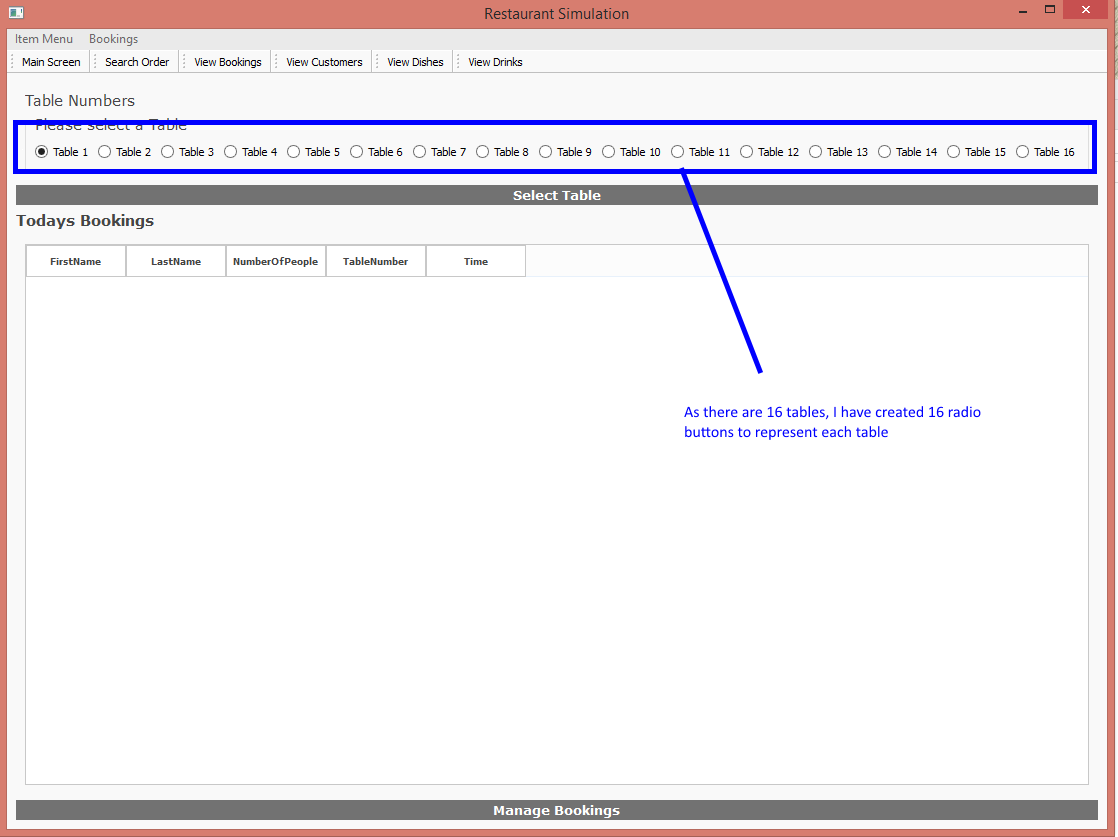
\includegraphics[width=\textwidth]{./Evaluation/images/radioButton}
    \caption{Main screen - highlighting the tables} \label{fig:radioButton}
\end{figure}

\subsubsection{Table shapes will be big so it won't be hard to click on them but not so big that 16 tables can fit on the GUI}
\begin{itemize}
	\item Objective has not been met
	\item I have used radio buttons to represent tables therefore I do not have any table shapes to meet this objective

\end{itemize}

\subsubsection{Clicking on table will bring up a window which shows the status such as the date and food items ordered with noticeable order modification options}
\begin{itemize} 
	\item Objective has mostly been met
	\item The user would have to select the table radio button and then click on Select Table
	\item The table has to be occupied to bring up the status window

\end{itemize}

\section{Effectiveness}

\subsection{Order alterations}
\subsubsection{Have clear Add, Delete and Create invoice buttons}
\begin{itemize}
	\item Objective has been met
	\item The application has clear Add and Delete buttons (User Questionnaire)
	\item  a

\end{itemize}


%include as many subsections as necessary for your objectives
\subsection{Objective Evaluation}

\section{Learnability}

\section{Usability}

\section{Maintainability}

\section{Suggestions for Improvement}

\section{End User Evidence}

\subsection{Questionnaires}

\subsection{Graphs}

\subsection{Written Statements}
